\documentclass[11pt]{article}

\usepackage[utf8]{inputenc}
\usepackage[T1]{fontenc}
\usepackage[margin=1in]{geometry}
\usepackage{graphicx}
\graphicspath{{./}{docs/}}
\usepackage{booktabs}
\usepackage{amsmath}
\usepackage{url}
\usepackage{xcolor}
\usepackage{enumitem}
\usepackage[hidelinks]{hyperref}

\title{Indic Speech Command Recognizer: Whisper-Tiny with Acoustic Wakeword and Multilingual Command Recognition}

\author{SMAI Assignment 3, Topic T11.7}
\date{}

\begin{document}
\maketitle

\begin{abstract}
We build a CPU-only multilingual speech-command frontend for SMAI Assignment 3
Topic T11.7. The system listens for the English wakeword ``Hey Bharat'' and
then recognises smart-home commands in Hindi, Tamil, and Telugu. The base
model is Whisper-tiny, whose weights are kept frozen. We compare two
recognition heads: Path A, a forced-language transcription and fuzzy-matching
pipeline, and Path B, a contrastive projection head over Whisper encoder
embeddings. Path B is the submitted recogniser because the assignment uses a
fixed Indic command set, and Path B gives higher command accuracy, lower
latency, and stronger hard-negative rejection. The final learned head reaches
93.22\% headline accuracy and 91.24\% $\pm$ 6.25\% 5-fold cross-validation
accuracy, while running on CPU.
\end{abstract}

\section{Links and Team}

\textbf{Repository:} \url{https://github.com/saiaditya14/smai-a3}\\
\textbf{Deployed prototype:} \url{https://engja9hyuz4sjstbxdka2e.streamlit.app/}

\begin{table}[h]
\centering
\caption{Team details}
\small
\begin{tabular}{lll}
\toprule
Name & Roll number & Email \\
\midrule
Aryan Maskara & 2023111004 & aryan.maskara@research.iiit.ac.in \\
Sai Ramanathan & 2023101096 & sai.ramanathan@students.iiit.ac.in \\
Neha Murthy & 2023115018 & neha.murthy@research.iiit.ac.in \\
Yajat Lakhanpal & 2023111015 & yajat.lakhanpal@research.iiit.ac.in \\
Prasoon Dev & 2023111014 & prasoon.dev@research.iiit.ac.in \\
Aanchal Mundhada & 2023112016 & aanchal.mundhada@research.iiit.ac.in \\
\bottomrule
\end{tabular}
\end{table}

\section{Introduction}

Smart-home and accessibility tools often assume fluent English. We instead
build a multilingual command recogniser that accepts an English wakeword and
then executes commands in Hindi, Tamil, or Telugu. The deployment constraint is
modest hardware: no GPU and no paid inference. We therefore use Whisper-tiny
(39M parameters) as a frozen acoustic and ASR backbone.

The contribution is a lightweight task adaptation around this frozen model.
A raw Whisper-tiny exact-match baseline reaches only about 3.7\% intent
accuracy on the command task. With an acoustic wakeword detector,
forced-language decoding, fuzzy command matching, and a learned contrastive
projection head, the final Path B recogniser reaches 93.22\% headline
accuracy on the fixed command set.

\section{Data}

\begin{table}[h]
\centering
\caption{Datasets and evaluation pools}
\begin{tabular}{lll}
\toprule
Source & Use & Size \\
\midrule
\texttt{data/<command>} & Real command clips & 149 clips \\
\texttt{data/<command>} + pitch shifts & Train-only command variants & 596 variants \\
\texttt{help/yes} + pitch shifts & Wakeword anchor variants & 24 variants \\
\texttt{help/no} + noise/time shifts & Reject-class variants & 104 variants \\
\texttt{help/no\_test} & Unseen hard negatives & 10 clips \\
\texttt{data/none} & Easy negatives & 100 clips \\
\texttt{FLEURS hi/ta/te} & ASR baseline & 1445 clips \\
\texttt{audio ablation} & Preprocessing stress tests & 447 runs \\
\bottomrule
\end{tabular}
\end{table}

The command corpus starts from 149 self-recorded clips. Following standard
speech-learning practice, we expand the training set with pitch-shifted
waveform variants and train a reject prototype using augmented hard negatives.
We report originals and augmented variants separately for transparency; the
augmentation is a valid part of the dataset pipeline, while all headline
command accuracies are still computed on real held-out recordings. Counting
FLEURS baselines, negative pools, augmentation, and the audio-preprocessing
ablation, the project processes over 2k audio examples/runs while keeping the
test clips separate from train-only variants.

The 149 command clips are the independent self-recorded command set: ten
smart-home commands, three Indic languages, and five takes per command-language
pair, with one missing/corrupt recording. Each take contains the full spoken
interaction, including the wakeword prefix and the command phrase. This is why
the Path B headline split is meaningful for the submitted setting: training
uses takes 1--3 and evaluation uses takes 4--5, so the model is tested on
unseen real recordings while still matching the fixed T11.7 language and
command inventory.

The augmentation choices are deliberately speech-specific rather than generic
noise injection only. Pitch shifts (-3, +3, +6 semitones) simulate speaker
pitch variation without changing the command label. The reject class receives
hard negatives with noise and time shifts, because the failure mode for a
wakeword system is not random silence but near-miss phrases that sound like
``Hey Bharat''. The preprocessing ablation reuses the same real command clips
under controlled signal transformations, so it measures robustness rather than
inflating the evaluation set.

\section{Method}

\subsection{Two-stage architecture}

The system first applies a wakeword gate. If the gate fires, audio is routed to
a command recogniser:
\[
\text{audio} \rightarrow \text{wakeword gate} \rightarrow
\text{recognition head} \rightarrow \text{action}.
\]
Both recognition heads share the same wakeword gate.

\subsection{Wakeword detection}

Whisper-tiny's decoder can hallucinate on short proper nouns, so we avoid text
decoding for wakeword detection. We extract a Whisper encoder embedding,
L2-normalise it, and compare it with a ``Hey Bharat'' anchor. The anchor is
the average of the positive wakeword recordings and pitch-shifted variants
(-3, +3, and +6 semitones). At inference we slide a 1.5s window with a 0.5s
hop and trigger when the maximum cosine similarity is at least 0.910.

We use a sliding window because the wakeword is only a short prefix of a
longer utterance. A full-clip embedding for ``Hey Bharat batti jalao'' mixes
the wakeword with the command and can dilute the cosine match. The 1.5s window
lets the detector score the local acoustic region containing only the wakeword.
The threshold was chosen to keep the gate useful in the deployed app, then the
command recogniser handles the harder problem of rejecting near-miss commands.

\subsection{Path A: transcription and fuzzy matching}

Path A forces Whisper decoding in Hindi, Tamil, and Telugu, then compares the
transcript against a curated command dictionary. Matching uses exact substring
checks followed by a sliding-window \texttt{SequenceMatcher} ratio threshold
of 0.7. This path is interpretable and easy to extend, but slow because it may
run the decoder three times per query.

The language forcing is important. Without it, Whisper-tiny often translates
Indic speech into English instead of transcribing the spoken Hindi/Tamil/Telugu
phrase. That behaviour is acceptable for general ASR demos, but it breaks a
dictionary command recogniser because the matcher expects native-script or
romanised command phrases.

\subsection{Path B: contrastive projection head}

Path B skips autoregressive decoding. It mean-pools the Whisper encoder
embedding and passes it through a learned MLP:
\[
384 \rightarrow 256 \rightarrow 128.
\]
The head is trained with margin contrastive loss:
\[
\mathcal{L} = y d^2 + (1-y)\max(0, m-d)^2,
\]
where $y=1$ for same-command pairs and $d$ is Euclidean distance in projected
space. The loss is vectorised over all pairs for tractable CPU training.

This projection head is the only supervised learned component. Whisper-tiny
itself is frozen. A reject prototype is also trained from hard negatives and
augmented variants, allowing the system to return no command for near-miss
inputs.

We evaluate Path B in three regimes. The headline split trains on takes 1--3
and evaluates on takes 4--5. A 5-fold cross-validation run estimates sampling
variance. A stricter cross-language hold-out trains on two languages and tests
on the third; this is intentionally difficult and exposes whether the learned
space is language-independent or mostly learns language-specific command
prototypes.

\section{Prototype}

The deployed Streamlit app exposes Path A, Path B, and a combined mode in the
sidebar. It accepts browser microphone input, displays wakeword state, and
shows the matched command and latency.

\begin{figure}[h]
\centering
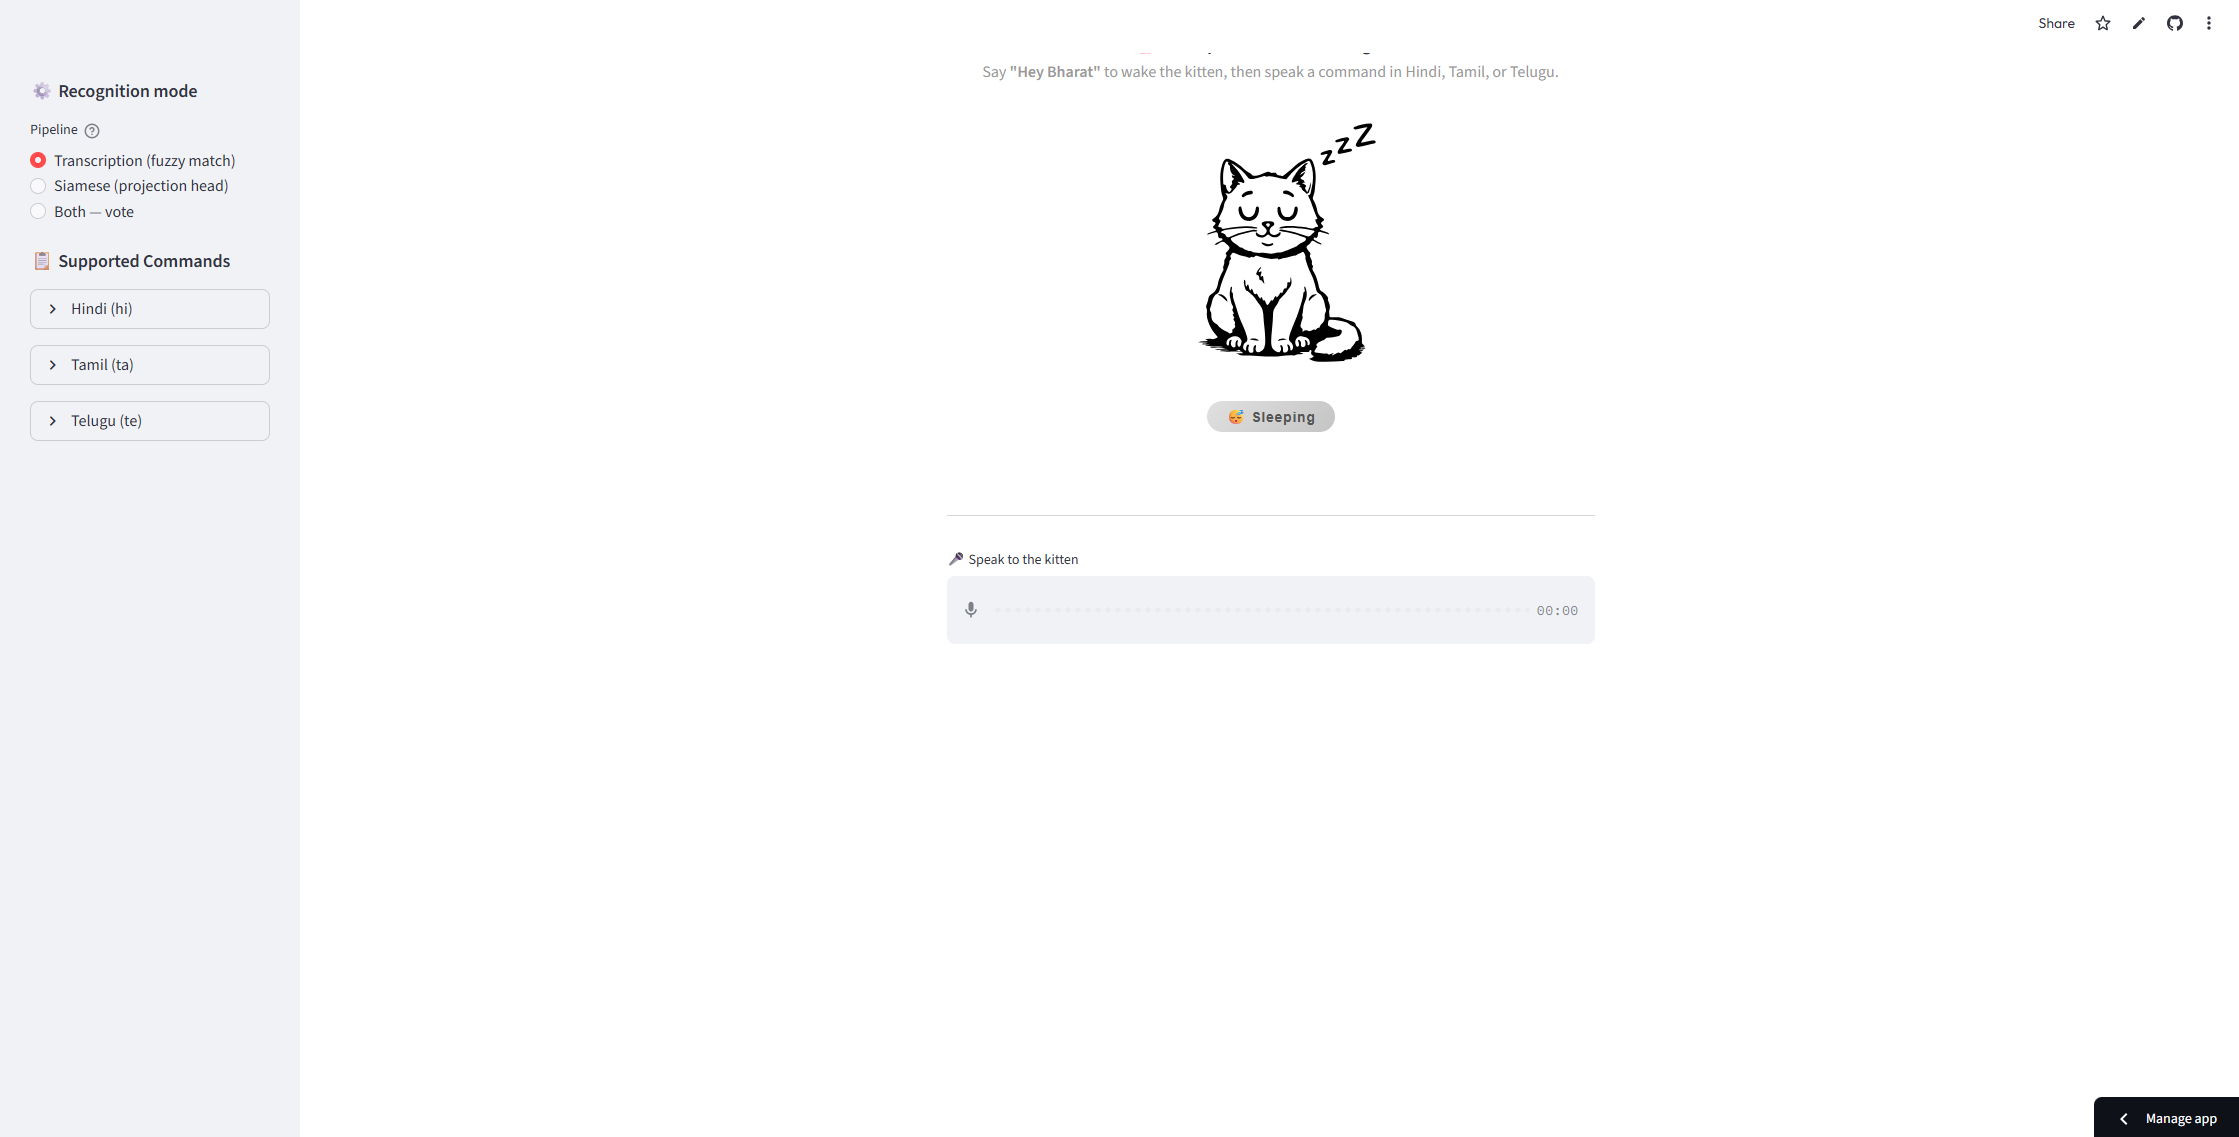
\includegraphics[width=0.45\textwidth]{screenshots/app_home_screen_r.png}
\caption{Home screen with recognition-mode sidebar.}
\end{figure}

\begin{figure}[h]
\centering
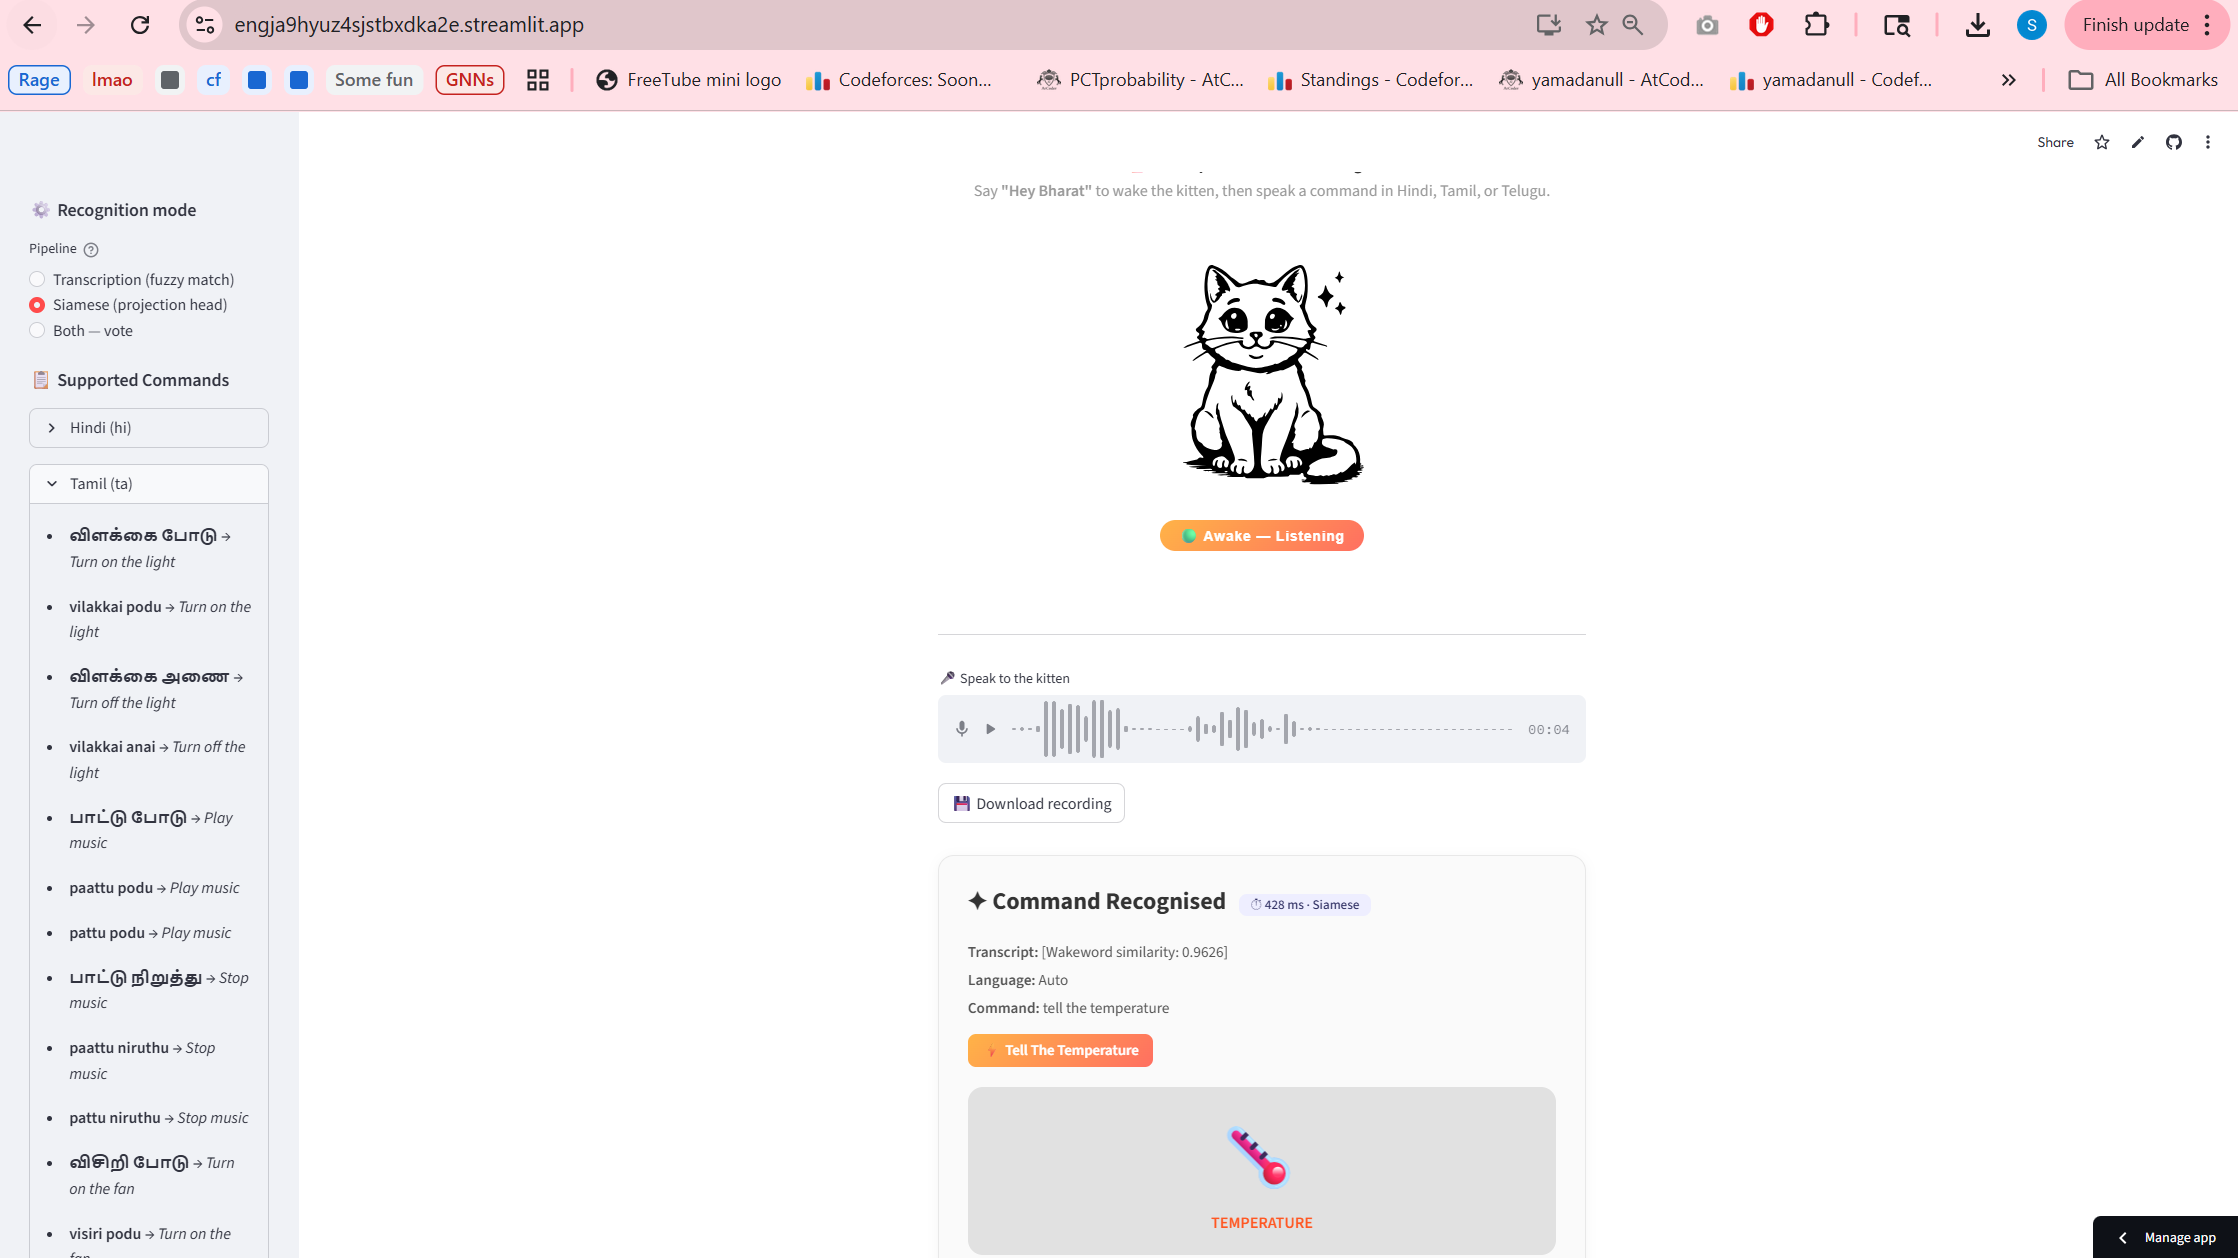
\includegraphics[width=0.45\textwidth]{screenshots/successful_detection.png}
\caption{Successful command detection in the deployed prototype.}
\end{figure}

\section{Results}

\subsection{FLEURS WER}

\begin{table}[h]
\centering
\caption{Whisper-tiny forced-language WER on FLEURS}
\begin{tabular}{lrr}
\toprule
Language & Samples & Avg. WER \\
\midrule
Hindi & 418 & 184\% \\
Tamil & 557 & 190\% \\
Telugu & 470 & 433\% \\
\bottomrule
\end{tabular}
\end{table}

WER exceeds 100\% because Whisper-tiny inserts extra text on short Indic
utterances. For intent recognition this is less damaging than raw WER
suggests, because fuzzy matching can tolerate phonetic spelling variation.
This result is also the reason we did not rely only on transcription. T11.7 is
an intent-recognition task after a wakeword, so a decoder transcript can be a
poor intermediate representation even when the acoustic features remain useful.

\subsection{Intent accuracy}

\begin{table}[h]
\centering
\caption{Intent recognition results}
\begin{tabular}{lll}
\toprule
System & Wake condition & Recognition accuracy \\
\midrule
Raw Whisper + exact match & no gate & 3.7\% \\
Path A: transcription + fuzzy & wake-gated & 43.62\% \\
Path A: transcription + fuzzy & skip-wake diagnostic & 70.47\% \\
Path B: projection head & wakeword-prefixed clips & 93.22\% \\
Path B: 5-fold CV & wakeword-prefixed clips & 91.24\% $\pm$ 6.25\% \\
\bottomrule
\end{tabular}
\end{table}

Path B is deployed behind the same wakeword gate as Path A. Its headline split
trains on takes 1--3 and evaluates on takes 4--5, so the recognition head is
tested on held-out real command recordings that include the wakeword prefix
but are not augmented evaluation copies.

\begin{table}[h]
\centering
\caption{Path B split analysis}
\begin{tabular}{lll}
\toprule
Evaluation & Train condition & Accuracy \\
\midrule
Headline & takes 1--3, eval takes 4--5 & 93.22\% \\
5-fold CV & stratified folds over real clips & 91.24\% $\pm$ 6.25\% \\
Cross-language hold-out & train two languages, test third & 0--18\% \\
\bottomrule
\end{tabular}
\end{table}

The cross-language result is intentionally reported even though it is weak.
It shows that the projection head is excellent for the fixed submitted
language set, but it should not be sold as zero-shot intent transfer to a new
Indic language. For a new language, Path A can be extended by adding dictionary
entries, while Path B needs new recordings and retraining.

\subsection{False positives}

\begin{table}[h]
\centering
\caption{False-positive rates on negative pools}
\begin{tabular}{lrrrr}
\toprule
Pool & n & Wake FPR & Path A cmd FPR & Path B cmd FPR \\
\midrule
\texttt{data/none} & 100 & 3.0\% & 2.0\% & 3.0\% \\
\texttt{help/no} & 26 & 69.2\% & 3.8\% & 0.0\% \\
\texttt{help/no\_test} & 10 & 50.0\% & 20.0\% & 0.0\% \\
\bottomrule
\end{tabular}
\end{table}

The wakeword gate is intentionally permissive; the second-stage recogniser is
responsible for suppressing command false positives. Path B's reject prototype
removes command firing on both seen and unseen hard negatives.

\subsection{Latency and architecture choice}

\begin{table}[h]
\centering
\caption{Path A vs Path B}
\begin{tabular}{lll}
\toprule
Metric & Path A & Path B \\
\midrule
Accuracy & 70.47\% & 93.22\% \\
Latency & $\sim$1830 ms & $\sim$730 ms \\
Hard-negative FPR & 20.0\% & 0.0\% \\
Add command & edit dictionary & retrain head \\
Add language & edit dictionary & collect data + retrain \\
\bottomrule
\end{tabular}
\end{table}

These latencies were measured on roughly 3--4 second command recordings. Path
A can be slower on longer recordings because it may run the autoregressive
decoder once per language, while Path B uses a single encoder pass and nearest
prototype lookup. For the submitted T11.7 prototype, Path B is the default
because the command set and target languages are fixed. Path A remains useful
as a fallback and debug path, especially when a recording contains only the
wakeword or when a future command/language must be added without retraining.

\section{Ablations}

\subsection{Language forcing and fuzzy matching}

\begin{table}[h]
\centering
\caption{Path A transcription ablation}
\begin{tabular}{lr}
\toprule
Configuration & Intent accuracy \\
\midrule
Raw Whisper-tiny + exact match & 3.7\% \\
Forced-language decode + fuzzy match & 70.47\% \\
\bottomrule
\end{tabular}
\end{table}

This ablation isolates the value of task-aware post-processing. The baseline
asks Whisper-tiny for a transcript and then exact-matches the output. It fails
because the model often translates Indic speech into English, emits extra
tokens, or changes romanised spellings. Forcing Hindi, Tamil, and Telugu
decoding and using a sliding-window fuzzy matcher raises skip-wake command
accuracy to 70.47\%. This is still slower and less accurate than Path B, but
it is a strong interpretable fallback.

\subsection{Audio preprocessing}

This was a deliberately negative-control style ablation. Our hypothesis was
that telephony-style preprocessing might help short voice commands by removing
high-frequency room noise and forcing the signal into the speech band. This is
plausible because many speech systems are robust to 8 kHz audio, and because
our app records from browser/laptop microphones rather than studio equipment.
We therefore evaluated every real command clip under three controlled input
conditions:

\begin{enumerate}[leftmargin=*]
\item \textbf{Baseline:} load at 16 kHz and peak-normalise.
\item \textbf{8 kHz telephony round-trip:} downsample to 8 kHz, then resample
back to 16 kHz before Whisper. This removes frequencies above roughly 4 kHz.
\item \textbf{300--3400 Hz bandpass:} apply a strict speech-band Butterworth
filter before feature extraction.
\end{enumerate}

\begin{table}[h]
\centering
\caption{Audio preprocessing ablation}
\begin{tabular}{lrr}
\toprule
Preprocessing & Correct / total & Accuracy \\
\midrule
Baseline 16 kHz, peak-normalised & 102 / 149 & 68.5\% \\
8 kHz telephony simulation & 88 / 149 & 59.1\% \\
Bandpass 300--3400 Hz & 101 / 149 & 67.8\% \\
\bottomrule
\end{tabular}
\end{table}

The hypothesis was mostly wrong, which is itself useful. The 8 kHz round-trip
drops accuracy by 9.4 percentage points, suggesting that Whisper-tiny's
log-mel frontend still benefits from high-frequency texture for these short
Indic commands. The bandpass result is only 0.7 points below baseline, so mild
speech-band filtering is not catastrophic, but it also does not improve the
system. The final pipeline therefore keeps preprocessing simple: 16 kHz
resampling and peak normalisation. This ablation contributes 447 controlled
audio runs and directly informs the deployment choice rather than being a
cosmetic experiment.

\subsection{Frozen vs learned projection}

\begin{table}[h]
\centering
\caption{Projection-head ablation}
\begin{tabular}{lr}
\toprule
Embedding space & Headline accuracy \\
\midrule
Frozen Whisper encoder + prototype & 38.98\% \\
Learned contrastive projection head & 93.22\% \\
\bottomrule
\end{tabular}
\end{table}

The learned head gives a 54.2 percentage-point improvement over frozen
encoder prototypes. This is the core supervised task adaptation.

\subsection{Reject class and augmentation}

\begin{table}[h]
\centering
\caption{Reject-class ablation}
\begin{tabular}{lrr}
\toprule
Configuration & Headline acc. & Hard-negative FPR \\
\midrule
No reject class, no command pitch augmentation & 88.14\% & 80\% \\
Reject class + command pitch augmentation & 93.22\% & 0\% \\
Reject class on unseen \texttt{help/no\_test} & 93.22\% & 0\% \\
\bottomrule
\end{tabular}
\end{table}

This is the main robustness ablation for Path B. A nearest-prototype command
classifier will always choose some command unless it has a way to reject
near-miss audio. Training a reject prototype from hard negatives and augmented
variants both improves command accuracy and removes command firing on the hard
negative pools. The unseen \texttt{help/no\_test} result matters because those
clips were not used to train the reject prototype.

\section{Limitations}

First, the command-specific dataset starts from 149 independent recordings.
Augmentation is a valid speech-learning tool and is part of the training
pipeline, but the main barrier to production quality is still data scale and
coverage. A larger original corpus across many more speakers, accents,
microphones, rooms, background noises, speaking speeds, and near-miss negative
phrases would be the most reliable way to improve robustness. Second, the
wakeword threshold is fixed at 0.910 and was tuned on the team's recordings;
deployment on weaker laptop or browser microphones may benefit from a broader
calibration set. Third, Path B does not generalise well to held-out languages,
so adding a new Indic language requires new recordings and retraining. Fourth,
the wakeword gate is permissive on hard negatives; the submitted system relies
on the second-stage recogniser and reject prototype to suppress command false
positives. Finally, the system does not fine-tune Whisper-tiny itself. Future
work could train a LoRA adapter or a small wakeword-only classifier to decide
whether speech after the wakeword contains an actual command.

\section{Future Work}

The most direct next step is a stronger wakeword module. The current cosine
gate is simple and CPU-friendly, but a small binary classifier over Whisper
encoder embeddings could reduce hard-negative triggers while preserving recall
for real ``Hey Bharat'' utterances. A second lightweight classifier could
separate wakeword-only audio from wakeword-plus-command audio, preventing the
command head from over-interpreting bare wakeword clips.

The biggest production upgrade would be more data. The next collection round
should target both quantity and diversity: phone microphones, laptop
microphones, headsets, noisy rooms, different distances from the microphone,
soft/loud speech, fast/slow speech, multiple accents, more speakers per
language, longer conversational negatives, and wakeword-only clips. This would
make threshold calibration more reliable for the deployed app and would also
let the reject class learn a broader boundary around real non-command speech.
For model adaptation, a LoRA fine-tune of Whisper-tiny or a multilingual
projection head trained with more languages could improve Path A transcription
and reduce Path B's weak cross-language hold-out behaviour. Finally, the app
could log anonymised failure cases with user consent so that future retraining
focuses on real deployment errors rather than only synthetic perturbations.

\section{Conclusion}

The final system shows that a frozen, CPU-only Whisper-tiny backbone can be
adapted into a useful Indic speech-command recogniser with lightweight
engineering and a small learned projection head. Path B is the submitted
recogniser because it is faster and more accurate for the fixed T11.7 command
setting, while Path A remains a practical fallback for interpretability and
future extensibility.

\section*{Acknowledgements}

Self-recordings were contributed by team members across Hindi, Tamil, and
Telugu speakers. Claude was used for code scaffolding, refactoring support,
and report drafting. All evaluation runs and conclusions are our own.

\begin{thebibliography}{4}
\bibitem{whisper}
A. Radford et al., ``Robust Speech Recognition via Large-Scale Weak
Supervision,'' 2022.
\bibitem{fleurs}
A. Conneau et al., ``FLEURS: Few-shot Learning Evaluation of Universal
Representations of Speech,'' 2022.
\bibitem{contrastive}
R. Hadsell, S. Chopra, and Y. LeCun, ``Dimensionality Reduction by Learning
an Invariant Mapping,'' CVPR, 2006.
\bibitem{jiwer}
M. Morris et al., \textit{jiwer}: Word Error Rate utility for Python.
\end{thebibliography}

\end{document}
